%!TeX root=../pridetop.tex

\chapter[Chapter \thechapter]{}
	
	 \makeatletter
\@ifclasswith{scrbook}{a5paper}
{%
	\begin{figure}[t!]
		\centering
		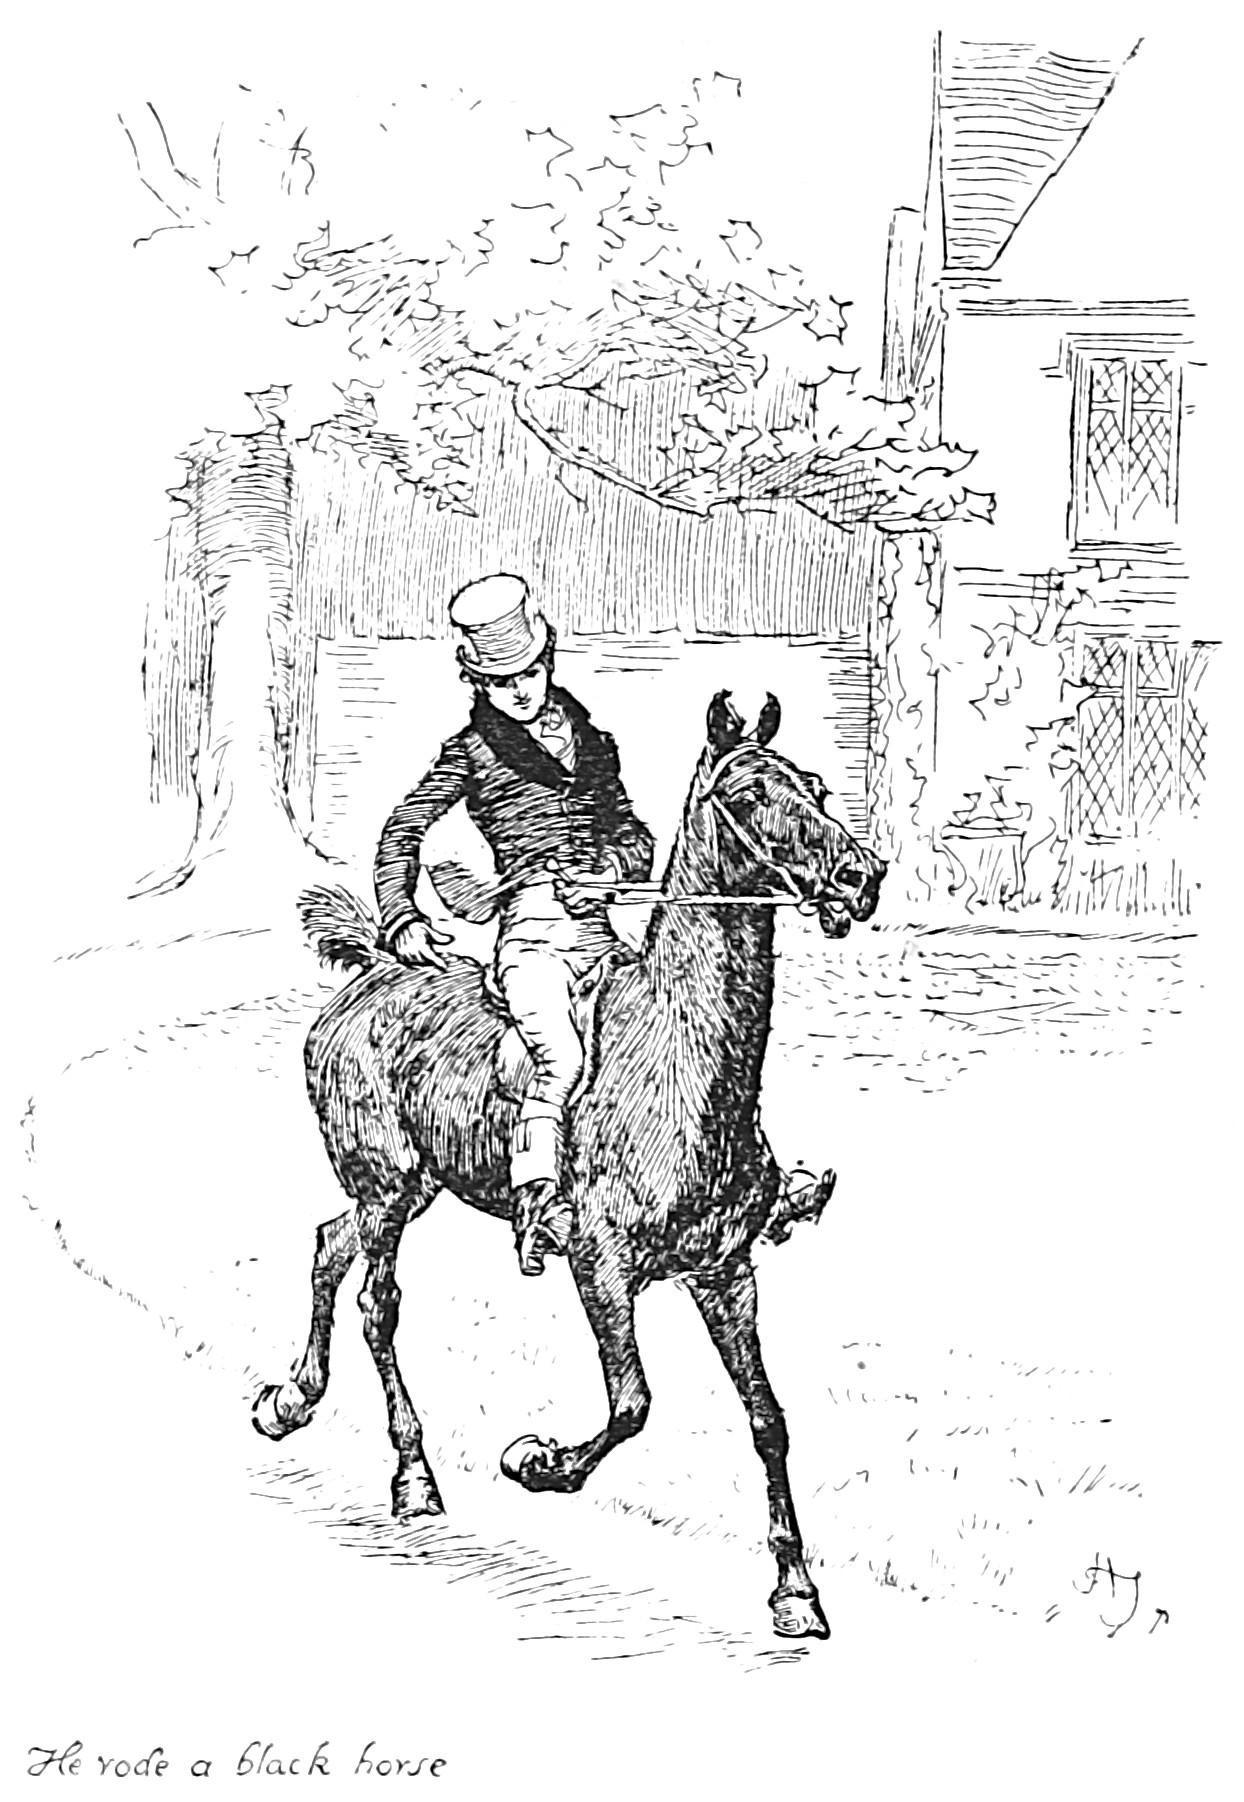
\includegraphics[width=.7\linewidth]{3blackhorse}
		\captionlistentry{He rode a black horse}
	\end{figure}
}{
	\begin{figure}[t!]
		\centering
		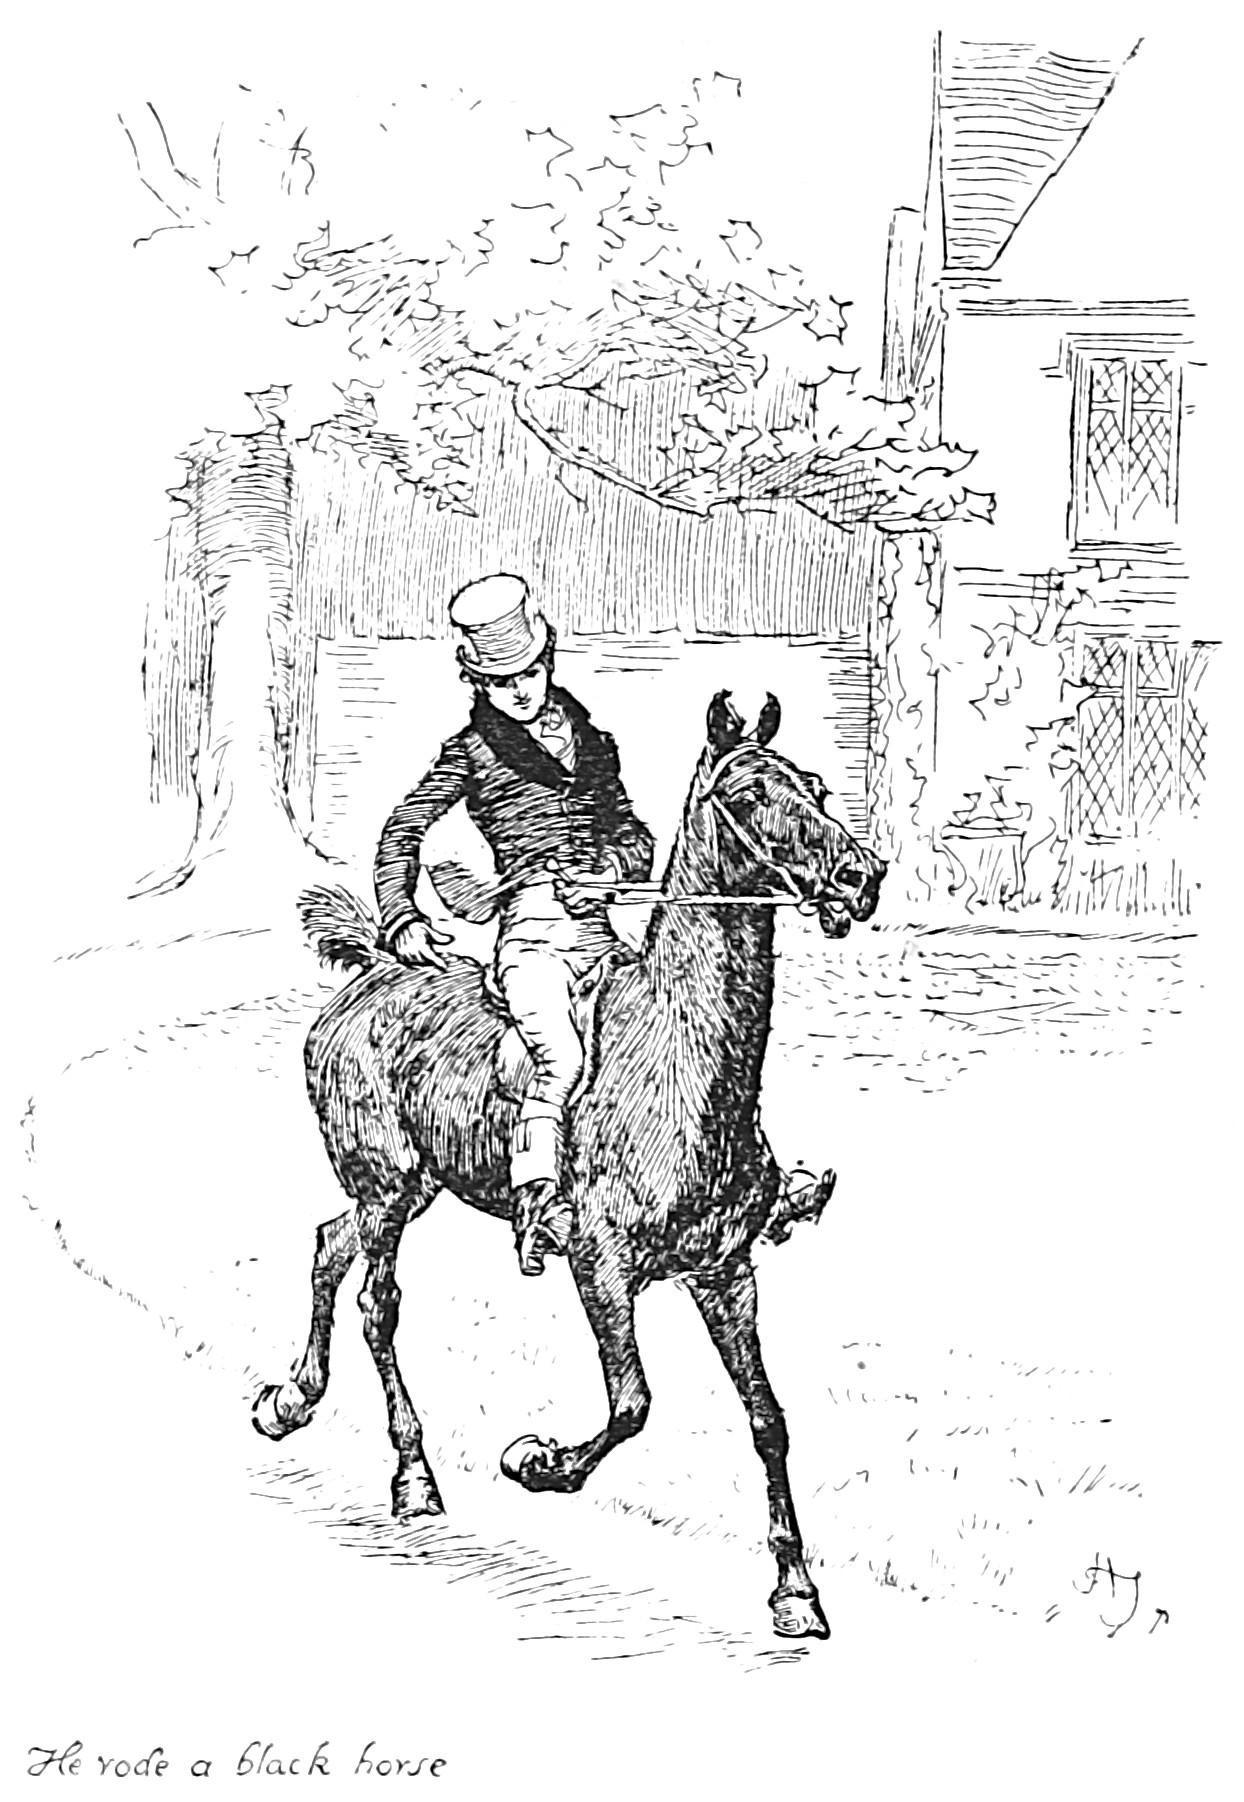
\includegraphics[width=.7\linewidth]{3blackhorse}
		\captionlistentry{He rode a black horse}
	\end{figure}
}

\makeatother

\lettrine[lines=6,image=true]{initials/chap3n}{ot} all that Mrs Bennet, however, with the assistance of her five daughters, could ask on the subject, was sufficient to draw from her husband any satisfactory description of Mr Bingley. They attacked him in various ways, with barefaced questions, ingenious suppositions, and distant surmises; but he eluded the skill of them all; and they were at last obliged to accept the second-hand intelligence of their neighbour, Lady Lucas. Her report was highly favourable. Sir William had been delighted with him. He was quite young, wonderfully handsome, extremely agreeable, and, to crown the whole, he meant to be at the next assembly with a large party. Nothing could be more delightful! To be fond of dancing was a certain step towards falling in love; and very lively hopes of Mr Bingley's heart were entertained.

»If I can but see one of my daughters happily settled at Netherfield,« said Mrs Bennet to her husband, »and all the others equally well married, I shall have nothing to wish for.«

In a few days Mr Bingley returned Mr Bennet's visit, and sat about ten minutes with him in his library. He had entertained hopes of being admitted to a sight of the young ladies, of whose beauty he had heard much; but he saw only the father. The ladies were somewhat more fortunate, for they had the advantage of ascertaining, from an upper window, that he wore a blue coat and rode a black horse.

\begin{figure}[tbh]
\centering
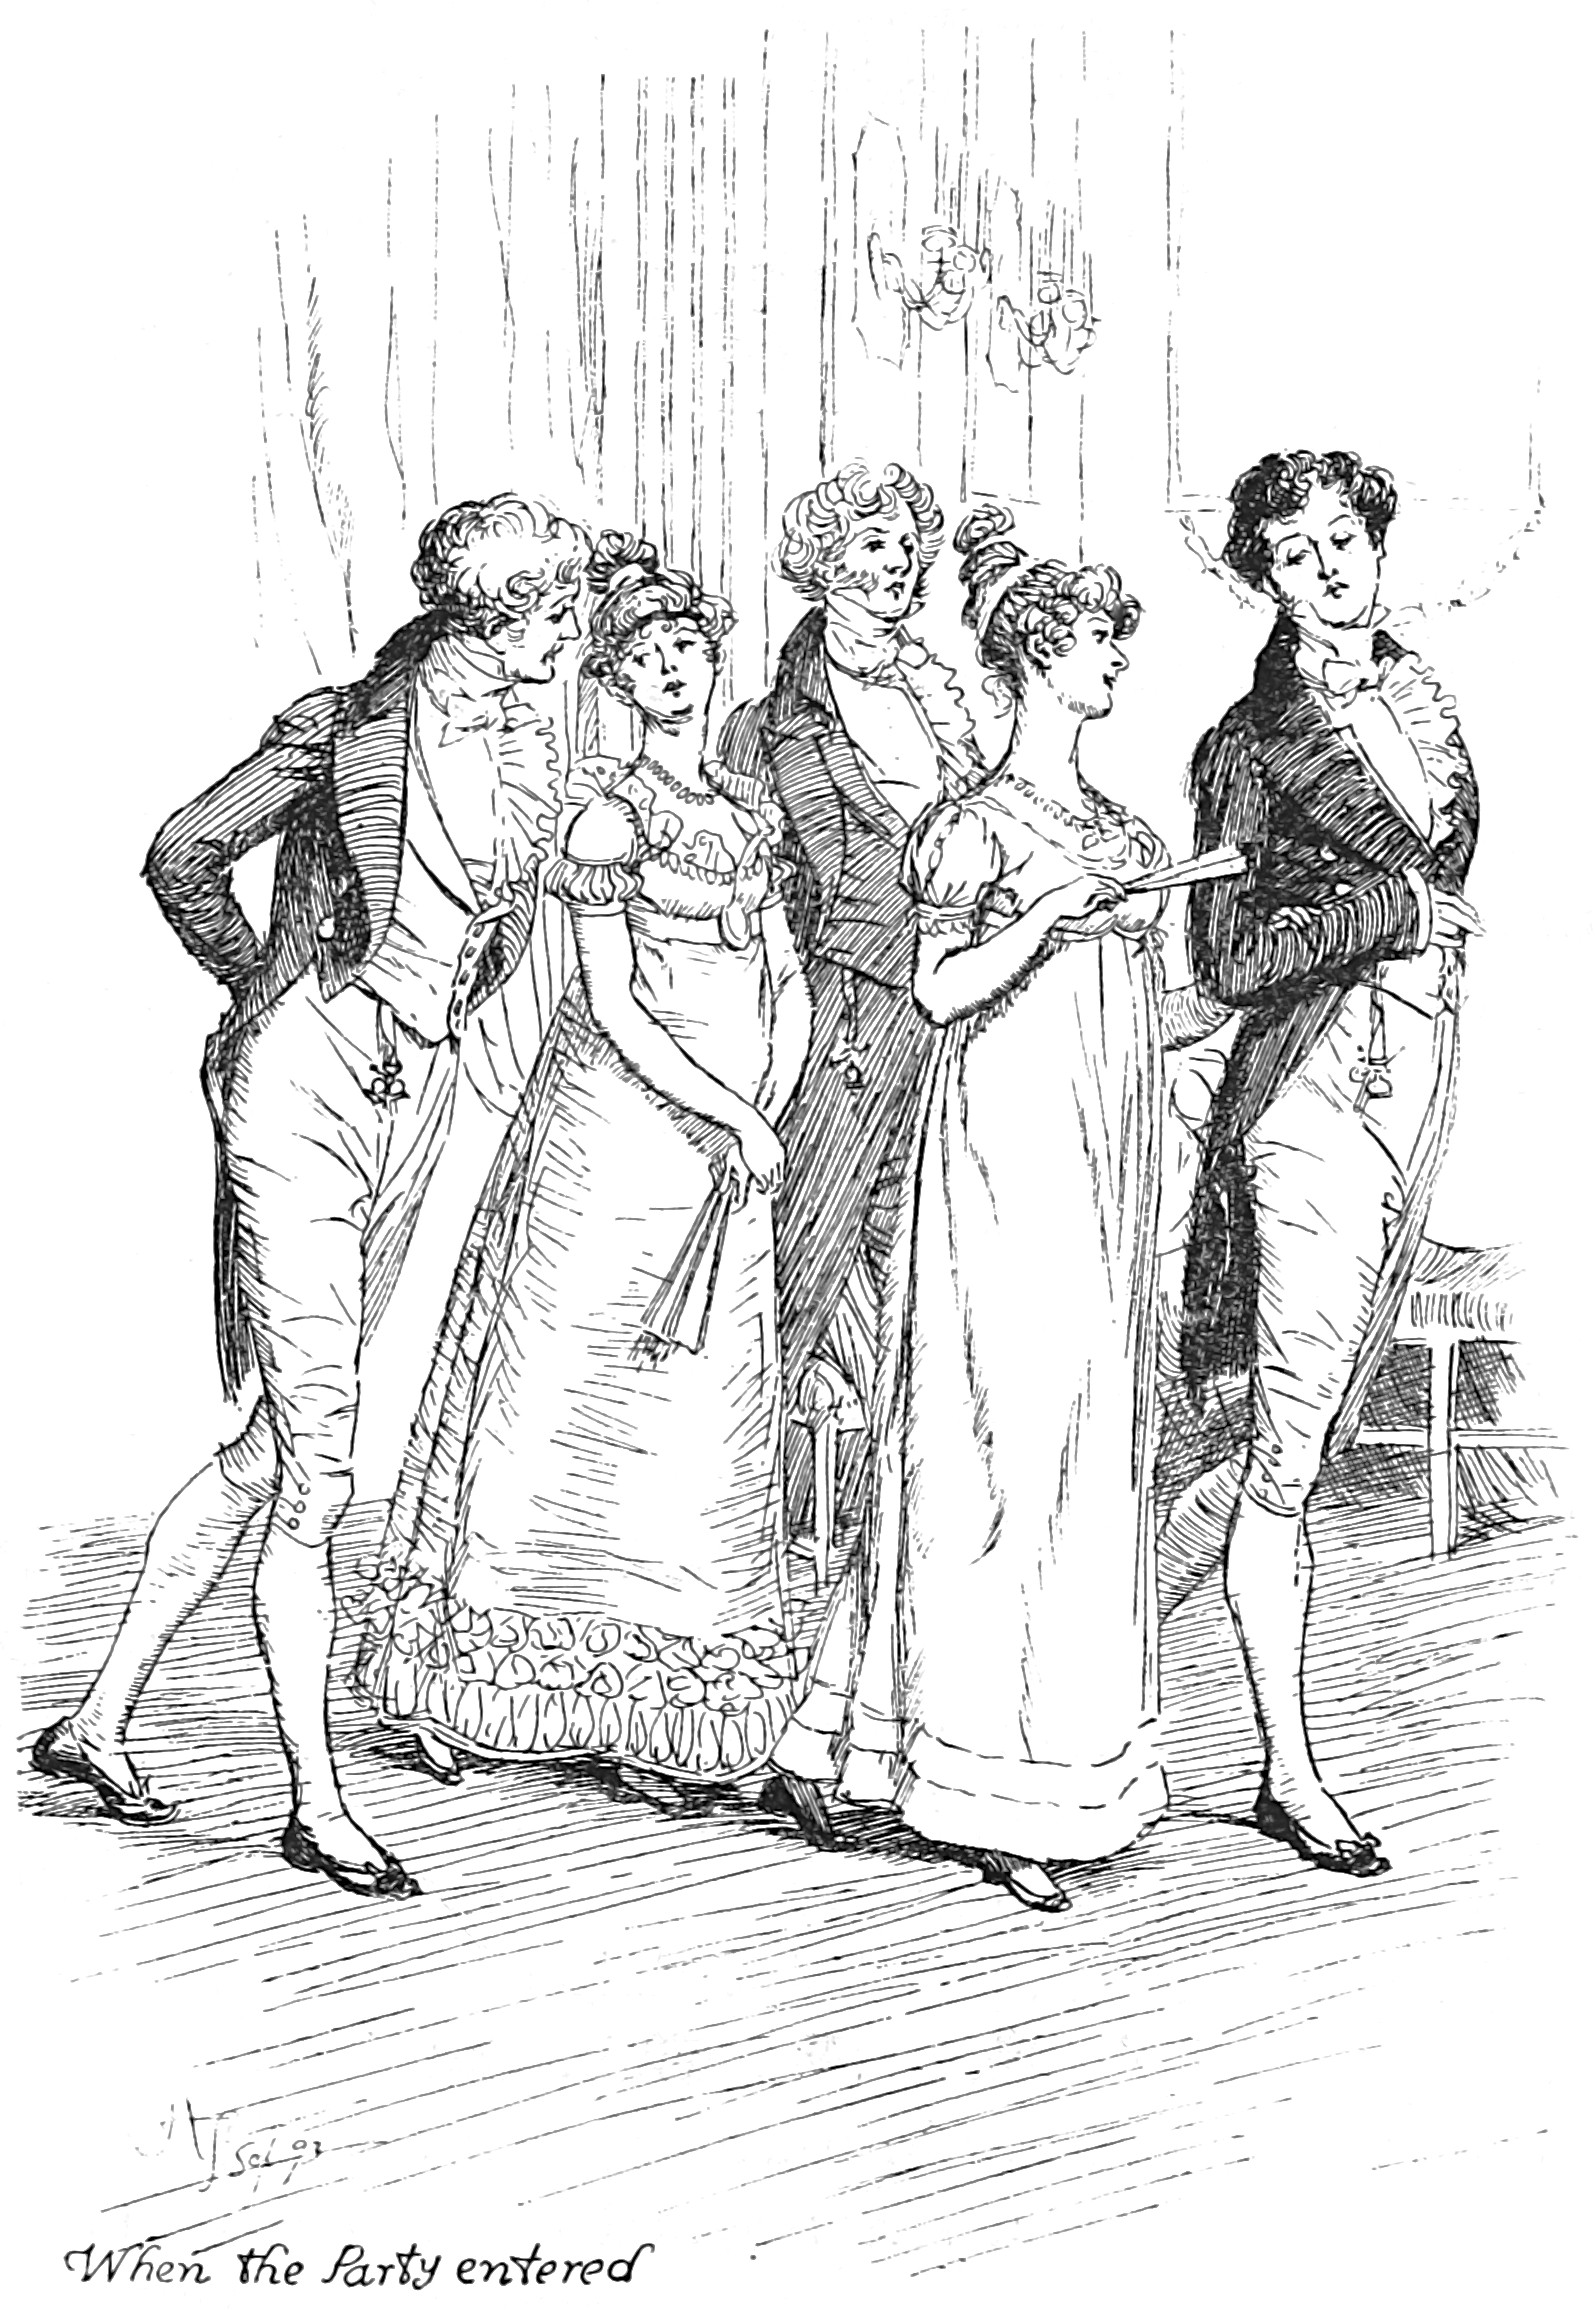
\includegraphics[width=.7\linewidth]{3partyentered}
\captionlistentry{When the party entered}
\end{figure}

An invitation to dinner was soon afterwards despatched; and already had Mrs Bennet planned the courses that were to do credit to her housekeeping, when an answer arrived which deferred it all. Mr Bingley was obliged to be in town the following day, and consequently unable to accept the honour of their invitation, etc. Mrs Bennet was quite disconcerted. She could not imagine what business he could have in town so soon after his arrival in Hertfordshire; and she began to fear that he might always be flying about from one place to another, and never settled at Netherfield as he ought to be. Lady Lucas quieted her fears a little by starting the idea of his being gone to London only to get a large party for the ball; and a report soon followed that Mr Bingley was to bring twelve ladies and seven gentlemen with him to the assembly. The girls grieved over such a number of ladies; but were comforted the day before the ball by hearing that, instead of twelve, he had brought only six with him from London, his five sisters and a cousin. And when the party entered the assembly-room, it consisted of only five altogether: Mr Bingley, his two sisters, the husband of the eldest, and another young man.

Mr Bingley was good-looking and gentlemanlike: he had a pleasant countenance, and easy, unaffected manners. His sisters were fine women, with an air of decided fashion. His brother-in-law, Mr Hurst, merely looked the gentleman; but his friend Mr Darcy soon drew the attention of the room by his fine, tall person, handsome features, noble mien, and the report, which was in general circulation within five minutes after his entrance, of his having ten thousand a year. The gentlemen pronounced him to be a fine figure of a man, the ladies declared he was much handsomer than Mr Bingley, and he was looked at with great admiration for about half the evening, till his manners gave a disgust which turned the tide of his popularity; for he was discovered to be proud, to be above his company, and above being pleased; and not all his large estate in Derbyshire could save him from having a most forbidding, disagreeable countenance, and being unworthy to be compared with his friend.

Mr Bingley had soon made himself acquainted with all the principal people in the room: he was lively and unreserved, danced every dance, was angry that the ball closed so early, and talked of giving one himself at Netherfield. Such amiable qualities must speak for themselves. What a contrast between him and his friend! Mr Darcy danced only once with Mrs Hurst and once with Miss Bingley, declined being introduced to any other lady, and spent the rest of the evening in walking about the room, speaking occasionally to one of his own party. His character was decided. He was the proudest, most disagreeable man in the world, and everybody hoped that he would never come there again. Amongst the most violent against him was Mrs Bennet, whose dislike of his general behaviour was sharpened into particular resentment by his having slighted one of her daughters.



Elizabeth Bennet had been obliged, by the scarcity of gentlemen, to sit down for two dances; and during part of that time, Mr Darcy had been standing near enough for her to overhear a conversation between him and Mr Bingley, who came from the dance for a few minutes to press his friend to join it.

»Come, Darcy,« said he, »I must have you dance. I hate to see you standing about by yourself in this stupid manner. You had much better dance.«

»I certainly shall not. You know how I detest it, unless I am particularly acquainted with my partner. At such an assembly as this, it would be insupportable. Your sisters are engaged, and there is not another woman in the room whom it would not be a punishment to me to stand up with.«

»I would not be so fastidious as you are,« cried Bingley, »for a kingdom! Upon my honour, I never met with so many pleasant girls in my life as I have this evening; and there are several of them, you see, uncommonly pretty.«

»\textit{You} are dancing with the only handsome girl in the room,« said Mr Darcy, looking at the eldest Miss Bennet.

»Oh, she is the most beautiful creature I ever beheld! But there is one of her sisters sitting down just behind you, who is very pretty, and I dare say very agreeable. Do let me ask my partner to introduce you.«

\begin{figure}[tbh]
\centering
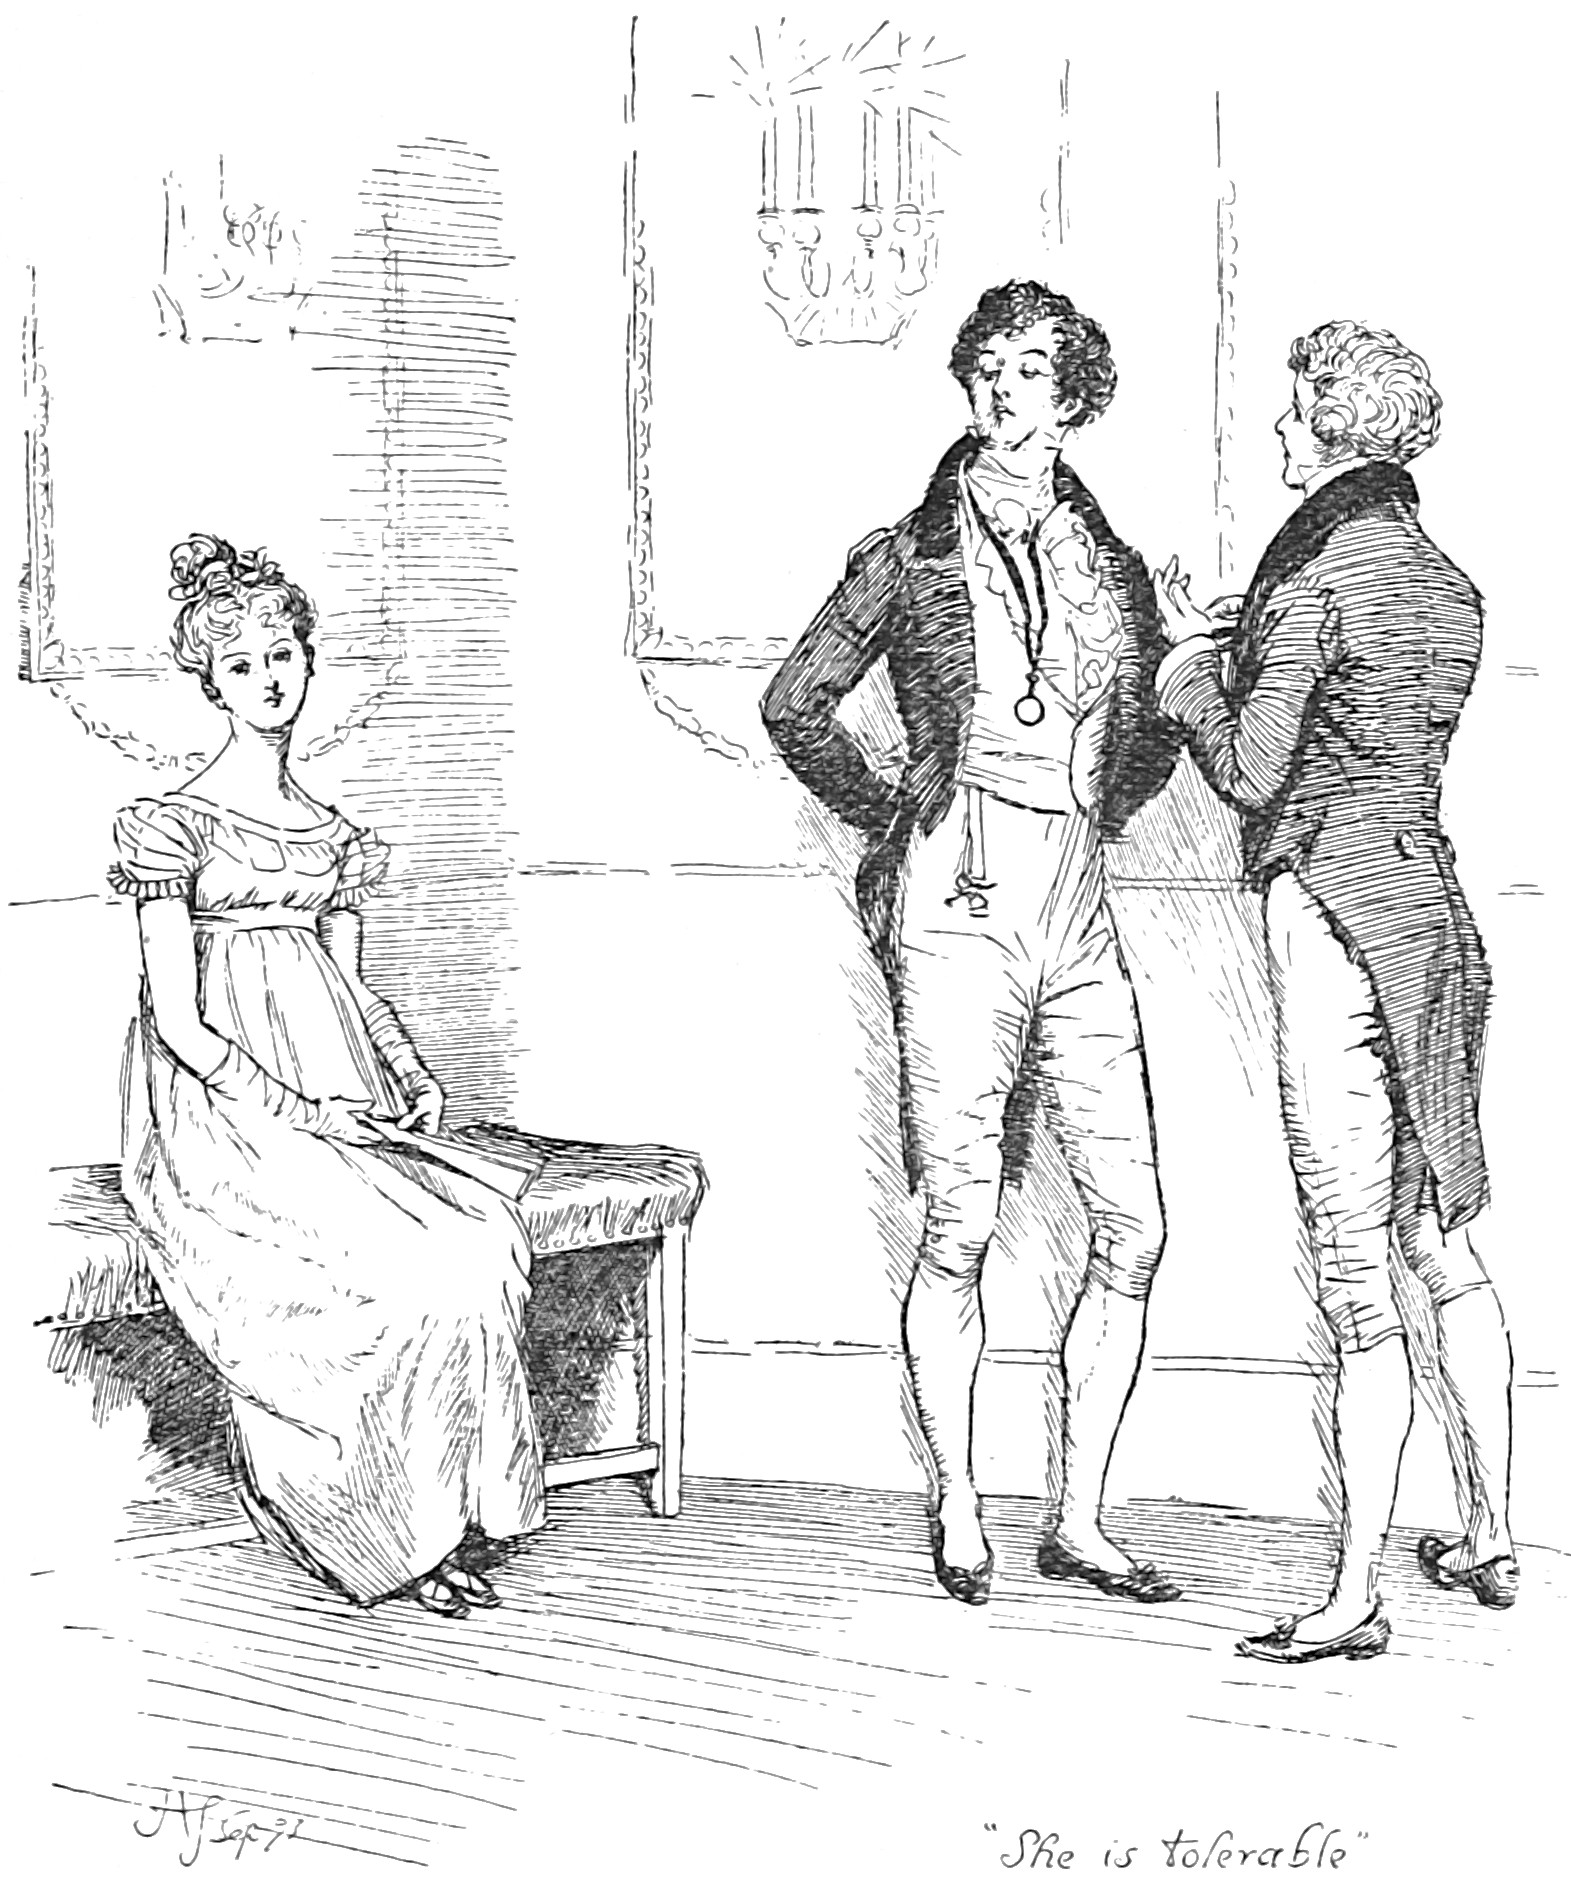
\includegraphics[width=.8\linewidth]{3tolerable}
\captionlistentry{»She is tolerable«}
\end{figure}

»Which do you mean?« and turning round, he looked for a moment at Elizabeth, till, catching her eye, he withdrew his own, and coldly said, »She is tolerable: but not handsome enough to tempt \textit{me}; and I am in no humour at present to give consequence to young ladies who are slighted by other men. You had better return to your partner and enjoy her smiles, for you are wasting your time with me.«



Mr Bingley followed his advice. Mr Darcy walked off; and Elizabeth remained with no very cordial feelings towards him. She told the story, however, with great spirit among her friends; for she had a lively, playful disposition, which delighted in anything ridiculous.

The evening altogether passed off pleasantly to the whole family. Mrs Bennet had seen her eldest daughter much admired by the Netherfield party. Mr Bingley had danced with her twice, and she had been distinguished by his sisters. Jane was as much gratified by this as her mother could be, though in a quieter way. Elizabeth felt Jane's pleasure. Mary had heard herself mentioned to Miss Bingley as the most accomplished girl in the neighbourhood; and Catherine and Lydia had been fortunate enough to be never without partners, which was all that they had yet learnt to care for at a ball. They returned, therefore, in good spirits to Longbourn, the village where they lived, and of which they were the principal inhabitants. They found Mr Bennet still up. With a book, he was regardless of time; and on the present occasion he had a good deal of curiosity as to the event of an evening which had raised such splendid expectations. He had rather hoped that all his wife's views on the stranger would be disappointed; but he soon found that he had a very different story to hear.

»Oh, my dear Mr Bennet,« as she entered the room, »we have had a most delightful evening, a most excellent ball. I wish you had been there. Jane was so admired, nothing could be like it. Everybody said how well she looked; and Mr Bingley thought her quite beautiful, and danced with her twice. Only think of \textit{that}, my dear: he actually danced with her twice; and she was the only creature in the room that he asked a second time. First of all, he asked Miss Lucas. I was so vexed to see him stand up with her; but, however, he did not admire her at all; indeed, nobody can, you know; and he seemed quite struck with Jane as she was going down the dance. So he inquired who she was, and got introduced, and asked her for the two next. Then, the two third he danced with Miss King, and the two fourth with Maria Lucas, and the two fifth with Jane again, and the two sixth with Lizzy, and the \textit{Boulanger}\longdash«

»If he had had any compassion for \textit{me},« cried her husband impatiently, »he would not have danced half so much! For God's sake, say no more of his partners. O that he had sprained his ancle in the first dance!«

»Oh, my dear,« continued Mrs Bennet, »I am quite delighted with him. He is so excessively handsome! and his sisters are charming women. I never in my life saw anything more elegant than their dresses. I dare say the lace upon Mrs Hurst's gown\longdash«

Here she was interrupted again. Mr Bennet protested against any description of finery. She was therefore obliged to seek another branch of the subject, and related, with much bitterness of spirit, and some exaggeration, the shocking rudeness of Mr Darcy.

»But I can assure you,« she added, »that Lizzy does not lose much by not suiting \textit{his} fancy; for he is a most disagreeable, horrid man, not at all worth pleasing. So high and so conceited, that there was no enduring him! He walked here, and he walked there, fancying himself so very great! Not handsome enough to dance with! I wish you had been there, my dear, to have given him one of your set-downs. I quite detest the man.«
